

\tikzset{every picture/.style={line width=0.75pt}} %set default line width to 0.75pt        

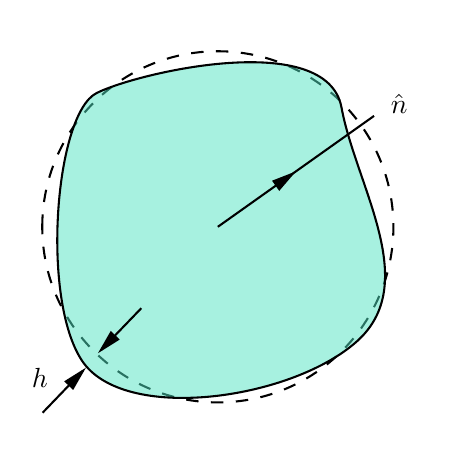
\begin{tikzpicture}[x=0.75pt,y=0.75pt,yscale=-1,xscale=1]
%uncomment if require: \path (0,300); %set diagram left start at 0, and has height of 300

%Shape: Circle [id:dp01917491317166009] 
\draw  [dash pattern={on 4.5pt off 4.5pt}] (121.52,175.11) .. controls (121.52,128.4) and (159.4,90.52) .. (206.11,90.52) .. controls (252.83,90.52) and (290.71,128.4) .. (290.71,175.11) .. controls (290.71,221.83) and (252.83,259.71) .. (206.11,259.71) .. controls (159.4,259.71) and (121.52,221.83) .. (121.52,175.11) -- cycle ;
%Shape: Polygon Curved [id:ds19124968571483536] 
\draw  [fill={rgb, 255:red, 80; green, 227; blue, 194 }  ,fill opacity=0.5 ] (147.71,110.66) .. controls (167.71,100.66) and (258.71,79.66) .. (265.71,117.66) .. controls (272.71,155.66) and (304.71,202.66) .. (272.71,230.66) .. controls (240.71,258.66) and (160.71,269.66) .. (140.71,239.66) .. controls (120.71,209.66) and (127.71,120.66) .. (147.71,110.66) -- cycle ;
%Straight Lines [id:da9840179317331423] 
\draw    (206.11,175.11) -- (281.38,121.67) ;
\draw [shift={(243.75,148.39)}, rotate = 504.62] [fill={rgb, 255:red, 0; green, 0; blue, 0 }  ][line width=0.08]  [draw opacity=0] (12,-3) -- (0,0) -- (12,3) -- cycle    ;
%Straight Lines [id:da9902953526542171] 
\draw    (121.71,264.66) -- (141.19,244.42) ;
\draw [shift={(142.58,242.98)}, rotate = 493.92] [fill={rgb, 255:red, 0; green, 0; blue, 0 }  ][line width=0.08]  [draw opacity=0] (12,-3) -- (0,0) -- (12,3) -- cycle    ;
%Straight Lines [id:da6416680662048091] 
\draw    (169.25,214.31) -- (149.76,234.55) ;
\draw [shift={(148.37,235.99)}, rotate = 313.91999999999996] [fill={rgb, 255:red, 0; green, 0; blue, 0 }  ][line width=0.08]  [draw opacity=0] (12,-3) -- (0,0) -- (12,3) -- cycle    ;

% Text Node
\draw (115,242) node [anchor=north west][inner sep=0.75pt]    {$h$};
% Text Node
\draw (287.96,109.72) node [anchor=north west][inner sep=0.75pt]    {$\hat{n}$};


\end{tikzpicture}
